\chapter{Implementierung}

Die Implementierung wird in zwei Teile gliedert, Learning Management System und  WebVR Applikation. Bei dem Teil LMS werden der Auswahl von LMS und die Erstellung des Unterrichts über der Vorbereitung einer Infusion erzählt. Bei dem Teil WebVR Applikation werden von Auswahl des Frameworks bis Implementierungen der Features, die beim Kapitel Konzeption gestaltet sind, erklärt.

\section{Learning Managment System Auswahl}

Viele LMS sind auf dem Markt angeboten. Eine geeignete Plattform für das Projekt wird ausgewählt, darauf ein Unterricht über Infusionsvorbereitung gestaltet wird. Paar Lernmethoden beispielsweise VR Übung werden in dem Unterricht eingesetzt.

 \subsection{LMS Auswahl}
 Laut Capterra stehen mehr als 400 LMS mit Web Applikation zu Verfügung. Jede LMS hat eigne Merkmale. Moodle ist ein LMS auf dem Markt, deren Eigenschaften sich an diesem Projekt gut anpassen.
 
 Der größte Vorteil von Moodle für das Projekt ist, dass Moodle eine kostenlos open source LMS Plattform ist. Das heißt, dass es möglich ist, die Moodle gratis auf eigenem Server zu installieren, mit eigener Datenbank zu verbinden und nach eigenen Anforderungen einzustellen.
 
 In Moodle können auch Arbeitsmaterialien wie Buch, Datei, Link usw. angeboten werden. Bei diesem Projekt wird der Benutzer durch den URLs in Moodle zu der WebVR Applikation geleitet, wie die erste Form, die in Konzeption beschrieben wird. 
 
 \subsection{Unterricht}
 Bei dem Unterricht Infusion Vorbereitung werden fünf Arbeitsmaterialien (drei Links, eine Datei und ein Textseite) und eine Aktivität eingesetzt. Die drei Links leiten jeweils auf einer Erklärung über Infusionsvorbereitung in Text, einer Erzählung über 5-R-Regel in Text und einem Video über Infusionsvorbereitung auf Youtube um. Die Datei ist ein Diagramm, damit der Ablauf der Vorbereitung einer Infusion graphisch dargestellt wird.
 
 Die Textseite bietet den Zugang der praktischen Übung in VR Umgebung. Die Methoden der Interaktion für unterschiedlichen Geräten werden zuerst informiert. Danach wird der Ablauf mit dem Diagramm noch einmal wiederholt. Und die acht Abschnitte in der Übung werden bezeichnet. Zum Abschluss werden acht Links aufgelistet, die auf dem entsprechenden Abschnitt in der VR Übung umleiten.
 
 Am Ende des Unterrichtes wird die Aktivität Test angeboten. Dadurch wird der Effekt des Lernens überprüft. Und das Ergebnis wird in Moodle gespeichert.
 
 Die VR Übung und der Test sind wiederholbar, um die Lernenden zu helfen, die Fertigkeit richtig zu beherrschen.
 
 image: Unterricht und Textseite ......... bis fertig von Unterricht
 
\section{WebVR Applikation}
Die Implementierung der WebVR Applikation ist der Schwerpunkt dieses Projektes. Zuerst Teil werden die Realisierungen, die das ganze Projekt betreffen, erzählt. Danach werden die Implementierungen für kleine Features erklärt.

 \subsection{Framework Auswahl}
 
 Um die Ziele dieses Projektes zu erreichen, muss das ausgewählte Framework folgende Anforderungen erfüllen:
 
 \begin{enumerate}
     \item Das Projekt kann gut mit LMS kommunizieren. Die Kommunikation kann durch URL oder Datenbank realisiert werden.
     \item Das Framework kann unterschiedliche Geräte unterstützen, z.B. PC, Smartphone und HMD.
     \item Das Projekt kann auf eigene Server bewahrt.
     \item Die Nutzung ist kostenlos.
     \item Reichliche Dokumentationen und erreichbare Community stehen zu Verfügung.
     \item Das Framework soll lange Zeit unterstützt und am besten kontinuierlich entwickelt werden.
 \end{enumerate}
 
 Im Kapitel Stand der Technik wird die Technologie der WebVR vorgestellt. Fünf Frameworks und Game Engines davon sind in der Lage, WebVR Applikation effizient zu entwickeln, nämlich , Unity, Play Canvas, Vizor, React 360 und A-Frame.
 
 \begin{itemize}
     \item \textbf{Unity} ist ein umfassende Game Engine. Viele built-in Funktionen stehen zu Verfügung. Mit das Plugin von Mozilla kann ein Projekt als WebVR Applikation exportiert werden. Allerdings wird das Projekt in einem Rahmen stellt. In diesem Rahmen ist die Entwicklung hoch effizient. Aber es ist schwierig, mit der Dinge außer dem Rahmen beispielsweise LMS anzupassen. Deswegen wird Unity nicht ausgewählt.
     \item \textbf{Play Canvas} ist ein webbasiert Game Engine. Damit kann das Projekt direkt als WebVR Applikation exportiert werden. Aber wenn man die Applikation auf eigne Server bewahren möchte, muss man monatlich zahlen.
     \item \textbf{Vizor} ist eine webbasierte visuelle WebVR Plattform. Die Scripts wird durch Blueprint geschrieben. Ihre Stärke ist, die 360 Grade oder VR Szene darzustellen. Allerdings reicht die Unterstützung für Interaktion für dieses Projekt nicht.
     \item \textbf{React 360} basiert teilweise auf three.js und wird von Facebook entwickelt. Die Logik der Entwicklung von React 360 ist gleich wie die bekannte JavaScript Bibliothek React im Bereich Frontend-Entwicklung. Allerdings wurde React 360 noch nicht vorgestellt, wenn dieses Projekt fängt an. Damals existierte nur der Vorfahr von React 360, nämlich React VR. Aber die Funktionalität von React VR war nicht reif genug, dieses Projekt zu entwickeln.
     \item \textbf{A-Frame} ist ein von Mozilla entwickeltes kostenloses open source WebVR Framework. Es bietet die größte Freiheit, das Projekt zu manipulieren. Außerdem werden unterschiedlichen Geräte unterstützt. Mit A-Frame werden die Funktionen von three.js in einem Entity-Component System eingewickelt. Die Features von three.js werden vererbt. Die Lösungen der Probleme über der Entwicklung können entweder in der Community von A-Frame oder der Community von three.js gefunden werden.
 \end{itemize}
 
\begin{figure}[ht]
\centering
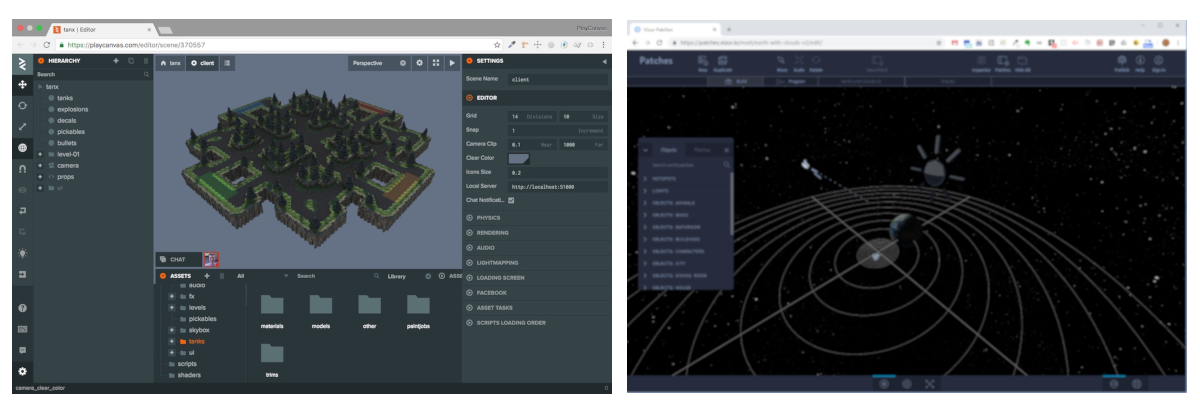
\includegraphics[width=\textwidth]{images/playCanvasVizor.png}
\caption[Webbasierte Engine]{Webbasierte Editoren von PlayCanvas und Vizor}
\label{fig:Webbasierte Engine}
\end{figure}

 A-Frame kann alle Anforderungen erfüllen. Deshalb wird nach dem Vergleich für A-Frame entschieden.
 
 \subsection{Projektierung}
 Im Bereich Web Entwicklung werden zwei beliebte Werkzeugen geboten, npm und Webpack. Mit den Beiden Werkzeugen kann Web Applikation projektiert werden und die Effizient der Entwicklung gefördert werden.
 
 NPM (Node Package Manager) ist ein Packetmanager für die JavaScript-Luafzeitumgebung Node.js. Mit npm ist es einfach, die auf npm gespeicherten Pakete(Softwares) zu benutzen. Die Abhängigkeit der Pakete wird durch npm automatisch behandelt. Alle benutzte Pakete werden in einer Datei eingepackt, sodass wird der Einsatz auf dem Server erleichtert.
 
 Webpack ist ein auf npm gespeichertes Werkzeug, die verwendete und geschriebene Dateien zu organisieren. Während der Entwicklung einer Web Applikation werden vielen Dateien beispielsweise Javascript Dateien, HTML Dateien, CSS Dateien, Bilder Dateien usw. benutzt. Die Dateien sind getrennt, aber mit einander verbindet. Solche dezentralisiere Struktur führt zum hohen Aufwand, das Projekt auf Server zu bewähren. Durch Webpack werden die Dateien während der Entwicklung bündig verpackt und komprimiert.
 
\begin{figure}[ht]
\centering
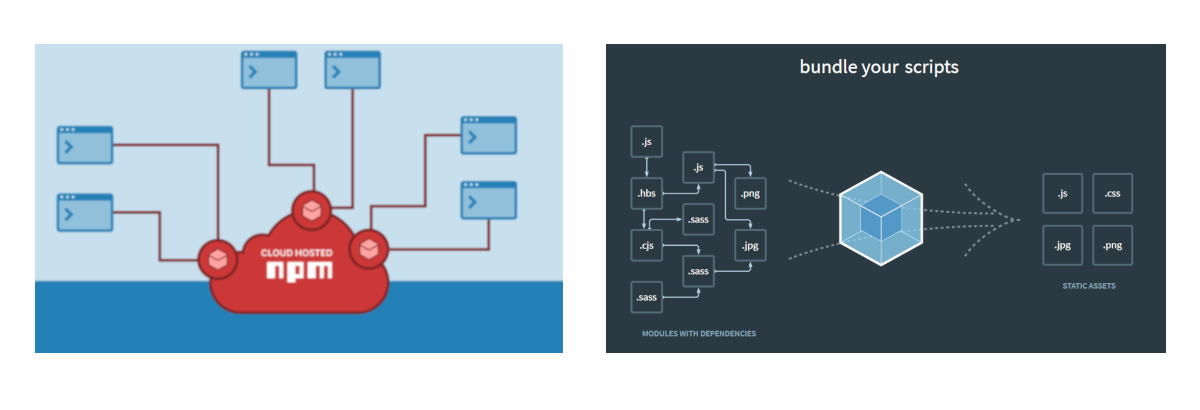
\includegraphics[width=\textwidth]{images/npmWebpack.png}
\caption[Projektierungswerkzeuge]{Projektierungswerkzeuge: NPM und Webpack}
\label{fig:npm Webpack}
\end{figure}
 
 Webpack-dev-server ist ein zusätzliches Werkzeug von Webpack. Dadurch wird die verpackte JavaScript Dateien automatisch kompiliert und die Webseite in Browser automatisch aktualisiert, solange die Codes geändert werden.
 
 Währen der Entwicklung einer Web Applikation können die CORS (Cross-Origin Resource Sharing) Errors auftauchen, wenn die lokale zugängliche Datei direkt in Browser aufgerufen wird, um das Effekt der Code anzuschauen. Der Grund ist, dass zur Sicherheit die Browsers Same-Origin-Policy benutzen. Das heißt, dass es untersagt wird, auf Objekte (zum Beispiel Grafiken) zuzugreifen, die von einer anderen Webseite stammen oder deren Speicherort nicht der Origin entspricht. Die von Browser direkt aufgerufenen lokalen Dateien gelten nicht als Same-Origin requests sondern Cross-Origin requests.
 
\begin{figure}[ht]
\centering
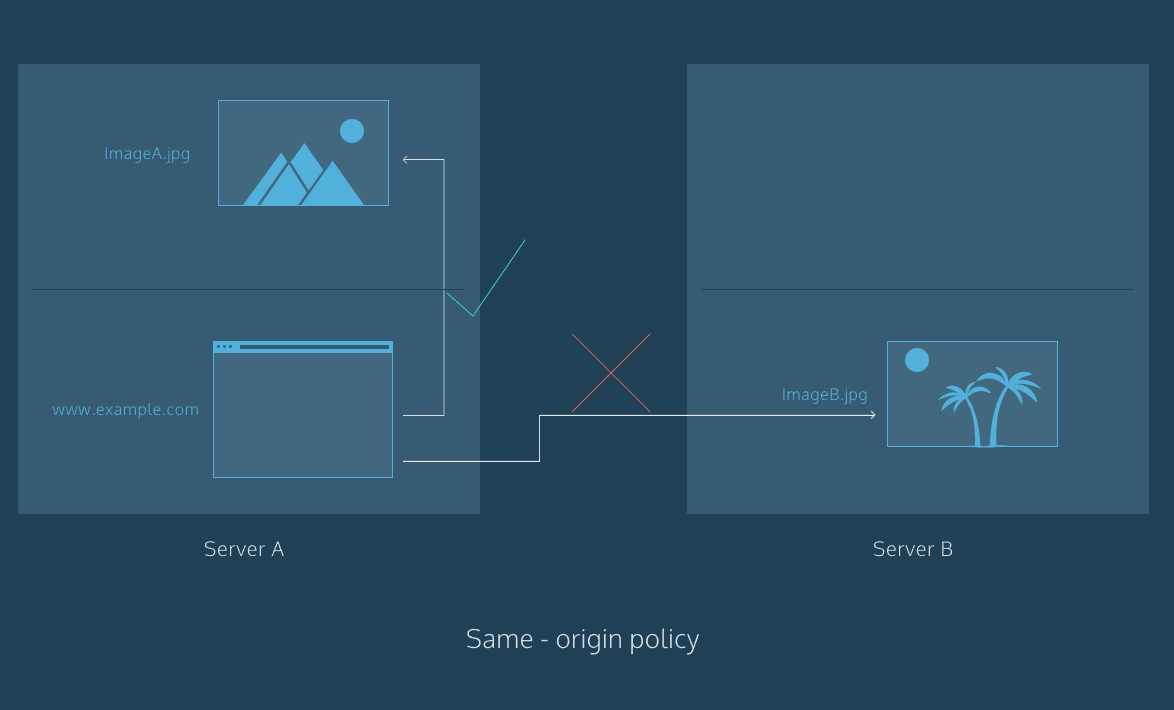
\includegraphics[width=\textwidth]{images/sameOrigin.png}
\caption[Same-Origin-Policy]{Same-Origin-Policy}
\label{fig:Same-Origin-Policy}
\end{figure}
 
 Http-server ist ein auf npm gespeichertes Werkzeug, dadurch ein Server (localhost) auf eigene PC erstellt werden kann. Und ein ausgewählter Ordner auf dem PC wird als das Wurzelverzeichnis des Servers eingerichtet. Alle Dateien in diesem Ordner gelten als in dem gleichen Origin, sodass die CORS Errors behoben werden.
 
 Nach der Projektierung ist die Struktur der Applikation wie Abbildung ~\ref{fig:projektStruktur} gezeigt.
 
\begin{figure}[ht]
\centering
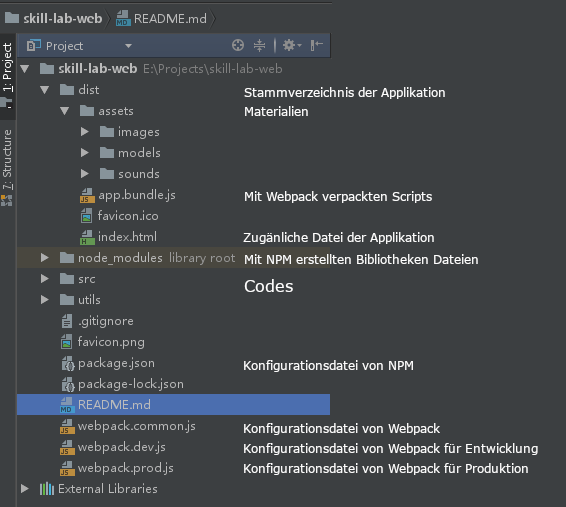
\includegraphics[width=\textwidth]{images/projektSturktur.png}
\caption[Struktur der Projekt]{Struktur der Projekt}
\label{fig:projektStruktur} 
\end{figure}
 
 \subsection{Zustände Management für Fortschritte}
 Im Kapitel Konzeption werden die Erkennung und Feedback Fortschritte erzählt. Wie werden die Fortschritte in der Applikation implementiert, wird in diesem Kapitel erklärt.
 
 Um die Fortschritte zu definieren, wird die Konzeption \glqq state container\grqq von der Technik Redux importiert. Jede Objekt in der VR Szene hat eigne Zustand, zum Beispiel Position. Die betreffenden Zustände werden geändert, wenn der Prozess der Applikation betrieben wird. Die Sammlung der Zustände der allen Objekten wird als \glqq state container\grqq bezeichnet. Durch die Kombination der Zustände wird der Fortschritt der Übung notiert.
 
 Eine Aktivität auf dem Objekt wird so durchgeführt. Zuerst wird die Interaktion auf einem Objekt erkannt. Danach werden die betreffenden Zustände geändert. Laut der Änderung der Zustände wird die entsprechende Aktivität des Objektes durchgeführt, was als Feedback an dem Benutzer gilt.
 
\begin{figure}[ht]
\centering
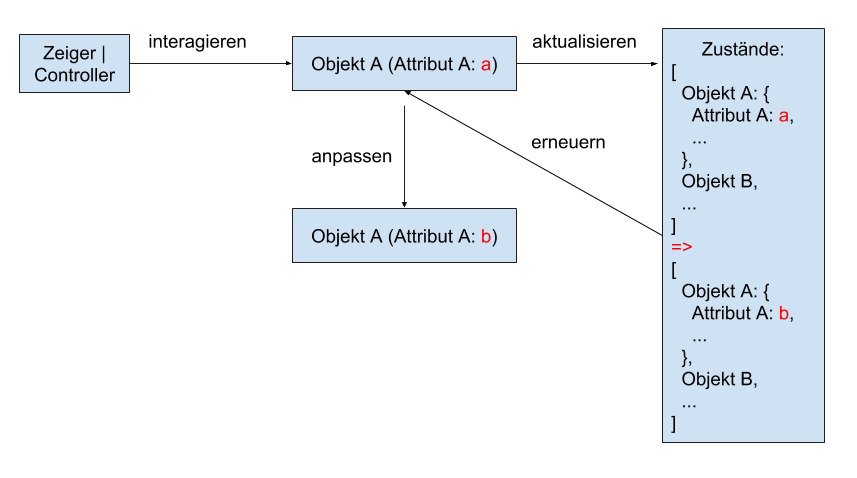
\includegraphics[width=\textwidth]{images/interaktionVerlauf.png}
\caption[Durchlauf einer Aktivität]{Durchlauf einer Aktivität}
\label{fig:interaktionVerlauf} 
\end{figure}
 
  \subsubsection{Beobachter (en. Observer Pattern)}
  Beobachter ist ein Entwurfsmuster (en. Design Pattern) aus dem Bereich Softwareentwicklung. Es ist geeignet, der Zustand Management zu implementieren.
  
  Die Funktionalität davon ist ähnlich wie der Mechanismus von Twitter. Zum Beispiel hat ein Fußballspieler einen Account von Twitter, damit er Nachrichten freigibt. Die Fans von dem Fußballspieler \glqq follow\grqq dem Fußballspieler auf Twitter. Wenn der Fußballspieler Nachrichten freigibt, werden die Fans benachrichtigt.
  
  Im Bereich Softwareentwicklung wird der Fußballspieler als \glqq Observable\grqq oder \glqq Subject\grqq bezeichnet. Die Fans werden als \glqq Observer\grqq bezeichnet. Die Aktivität \glqq follow\grqq ist \glqq Subscribe\grqq. Die Benachrichtigung heißt \glqq Notify\grqq.
  
\begin{figure}[ht]
\centering
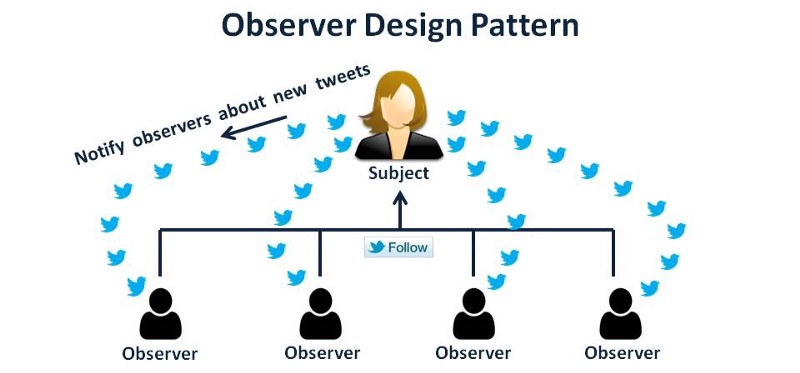
\includegraphics[width=\textwidth]{images/observerPattern.jpeg}
\caption[Observer Pattern]{Observer Pattern}
\label{fig:observerPatern} 
\end{figure}
  
  Um der das Oberserver Pattern zu implementieren, wird ein Class \glqq Observable\grqq in diesem Projekt erstellt.
  
\begin{figure}[ht]
\vspace*{0.3cm}
\centering
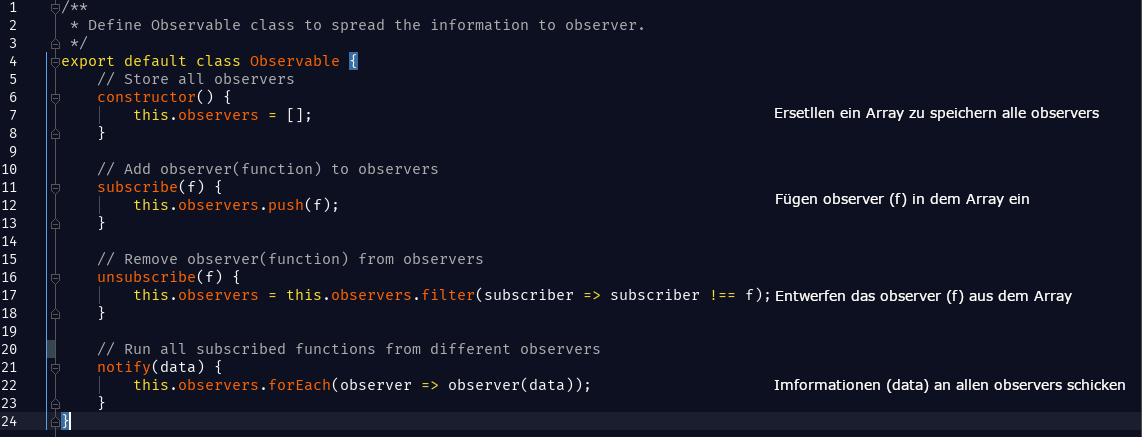
\includegraphics[width=\textwidth]{images/observable.png}
\caption[Class Observable]{Class Observale}
\label{fig:observable} 
\end{figure}
  
  Während der Erstellung einer \glqq Observable\grqq\ wird ein Array generiert, um die \glqq Observers\grqq\ zu speichern. Durch die Funktionen \glqq subscribe\grqq\ und \glqq unsubscribe\grqq\ können die \glqq Observers\grqq\ in dem Array eingefügt oder von dem Array ausgezogen werden. Die \glqq Observers\grqq\ (Funktionen) sollen ein Parameter haben, um die Nachrichten von \glqq Observer\grqq\ zu empfangen. Wenn die Funktion \glqq Notify\grqq\ aufgerufen wird, werden alle \glqq Observers\grqq\ in dem Array nacheinander aufgerufen. Der Parameter der Funktion \glqq Notify\grqq\ wird als Parameter der \glqq Observers\grqq\ eingesetzt, sodass die Nachrichten auszuteilen.
  
  \subsubsection{Zustände Management}
  
  Um das Zustand Management zu realisieren, wird ein Class \glqq stateIndex\grqq\ geschrieben. Da fast alle Objekt in der Szene mit diesem Class verbinden und das einzige \glqq state container\grqq referenzieren, wird das Class als \glqq static\grqq Class definiert.
  
  Mit \glqq init\grqq\ Funktion werden alle Zustände initialisiert. Die Initialisierung liegt an dem Query string in URL. Das Query string ist ein Teil von URL, dadurch der  Parameter bei dem \glqq request\grqq zusammen an dem Server geschickt. Bei dieser Applikation ist das Query string die Ziffer des ausgewählten Abschnitts. Mit dem Query string wird die Zustände nach dem Ausgewählten Abschnitt initialisiert.
  
  Während der Initialisierung wird eine Entität von Observable erstellt, um die Benachrichtigung vorzubereiten.
  
  Die \glqq init\grqq\ Funktion wird nur einmal durchgeführt, wenn die Applikation aufgerufen.
  
\begin{figure}[ht]
\centering
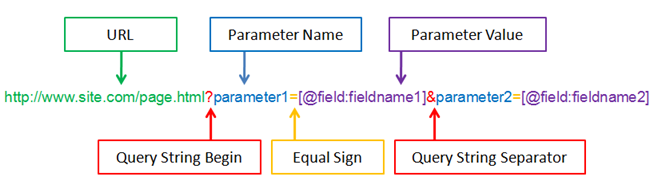
\includegraphics[width=\textwidth]{images/queryString.png}
\caption[Query String]{Query String}
\label{fig:queryString} 
\end{figure}
  
  Zu Sicherheit dürfen die Zustände von andere Objekt nicht erreichen. Deswegen werden die Funktionen von Class \glqq stateIndex\grqq\ angeboten, um die Zustände zu manipulieren.
  
  \begin{itemize}
      \item \textbf{getState}: alle aktuelle Zustände zu bekommen.
      \item \textbf{get}: bestimmte Zustand zu bekommen.
      \item \textbf{getIn}: bestimmte Zustand in tiefen Ebenen zu bekommen.
      \item \textbf{set}: bestimmte Zustand zu aktualisieren. Durch der Funktion \glqq Notify\grqq\ von \glqq Observable\grqq\ die neue Zustände an allen Observer auszuteilen.
      \item \textbf{setIn}: bestimmte Zustand in tiefen Ebenen zu aktualisieren. Durch der Funktion \glqq Notify\grqq\ von \glqq Observable\grqq\ die neue Zustände an allen Observer auszuteilen.
  \end{itemize}
  
 \subsection{Abschnitte Auswahl}
 Der Auswahl der Abschnitte kann auf zwei Zeitpunkten durchgeführt werden. Einer davon ist während der Aufruf der Applikation. Die Ziffer der ausgewählte Abschnitt wird durch dem Query string in URL an der Applikation gegeben. Der andere ist vor dem Nahm der Krankenakte in VR Szene. Auf dem Whiteboard werden die Abschnitte aufgelistet, dadurch bestimmter Abschnitt auswählen werden kann.
 
  \subsubsection{Abschnitte Auswahl durch URL}
  Die Zustände werden am Anfang als ursprüngliche Zustände initialisiert. Durch der Funktion \glqq getSectionSelectionFromURL\grqq\ in Class \glqq stateIndex\grqq\ kann die ausgewählte Ziffer bestimmen werden. Wenn die Ziffer zwischen 1 und 7 ist, werden die betreffenden Zustände durch die Funktion \glqq selectSection\grqq\ aktualisiert. Danach werden die Objekte in der Szene nach den Zuständen auch aktualisiert.
  
  Um die GUI richtig einzusetzen, wird ein Trick benutzt. Wenn die Applikation aufgerufen, wird die Szene nach den aktuellen Zuständen eingerichtet und werden gleichzeitig die Modells geladen. Es könnte passieren, dass das Modell noch nicht fertig geladen ist, wenn es von der Aktualisierung betroffen wird. Das führ zu Fehler der Applikation.
  
  Um das Problem zu lösen, wird die Ladung vor der Aktualisierung überprüft. Mit der Funktion \glqq setInterval\grqq\ wird es implementiert, jede 0,5 Sekunde die Zustand der Ladung zu überprüfen. Wenn alle Modells schon geladen ist, wird die Überprüfung beendet und die Szene aktualisiert.
  
\begin{figure}[ht]
\vspace*{0.3cm}
\centering
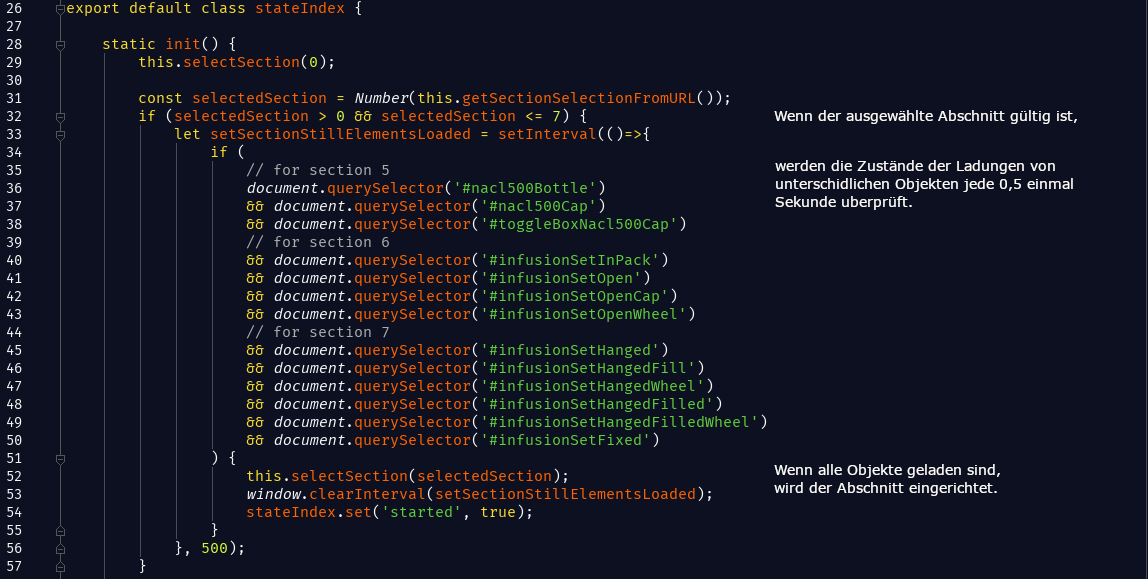
\includegraphics[width=\textwidth]{images/checkLadung.png}
\caption[Überprüfen die Zustände der Ladungen]{Überprüfen die Zustände der Ladungen}
\label{fig:checkLadung} 
\end{figure}
  
  \subsubsection{Abschnitte Auswahl in VR Szene}
  Auf dem Whiteboard werden die Abschnitte aufgelistet. Durch Zeiger oder Raycaster wird die Funktion \glqq selectSection\grqq\ in Class \glqq stateIndex\grqq\ mit entsprechendem Parameter aufgerufen, um der Abschnitt zu wechseln.
  
  Vor den Zeichnen auf dem Whitebard werden 7 \glqq toggle box\grqq eingesetzt, dadurch die Funktion \glqq selectSection\grqq\ von HTC Vive Controller aufgerufen kann.
  
\begin{figure}[ht]
\vspace*{0.3cm}
\centering
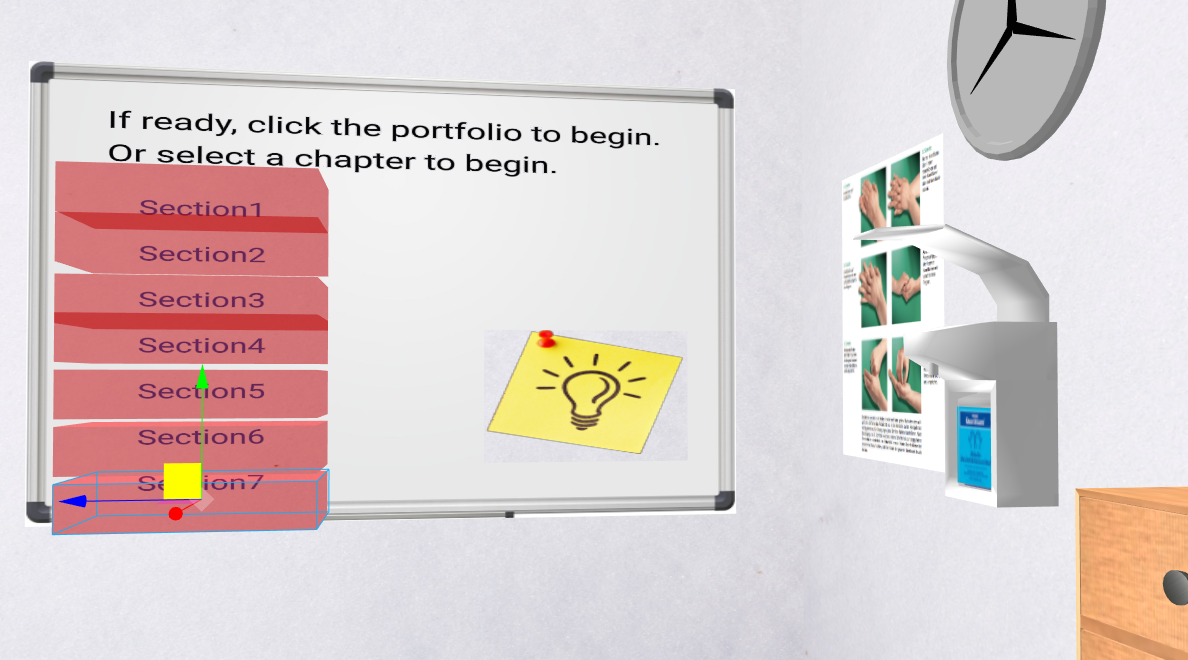
\includegraphics[width=\textwidth]{images/toggleBoxAbschnitte.png}
\caption[Toggle Boxes]{Toggle Boxes für Auswahl der Abscshnitte}
\label{fig:toggleBoxAbschnitte} 
\end{figure}
  
  \subsubsection{Möglichkeit der Verbesserung}
  Der Abschnitte Auswahl kann nicht nur während der Initialisierung, sondern auch nach der Initialisierung durchgeführt wird. Deswegen sollen die Funktionen über Abschnitte Auswahl wie \glqq selectSection\grqq\ nicht in Class \glqq stateIndex\grqq\ eingepackt werden, sondern in eigenen Datei geschrieben werden.
  
 \subsection{Gestaltung der Struktur von Class der Objekten}
 Um das Projekt effizient zu entwickeln, wird eine Struktur von Class gestaltet, die sich meisten Objekte in diesem Projekt anpassen kann. Die Struktur basiert auf die Class Struktur von A-Frame.
 
 \subsubsection{Gestaltung}
 Die Philosophie von A-Frame ist, mit spezifischen HTML Elements die Szene aufzubauen. Ein Element ist eine Kombination der Entitäten von unterschiedlichen Classes. Eine Entität kann ein HTML Element oder ein Attribut eines HTML Elements sein. Das Class in A-Frame wird als Component genannt.
 
 Drei Built-in Objekten von Component sind wichtig.
 \begin{itemize}
     \item \textbf{init} ist eine Funktion, die während der Erstellung einer Entität von Component durchgeführt wird.
     \item \textbf{schema} ist ein JavaScript Objekt, die Attribute von Component speichert.
     \item \textbf{update} ist eine Funktion, die durchgeführt wird, wenn das schema durch HTML geändert wird. Die Initialisierung gilt als eine Änderung von schema, d.h. dass die Funktion update während der Erstellung einer Entität durchgeführt wird. Deswegen muss die Funktion init nicht definiert, wenn die Funktion update existiert.
 \end{itemize}
 
\begin{figure}[ht]
\vspace*{0.3cm}
\centering
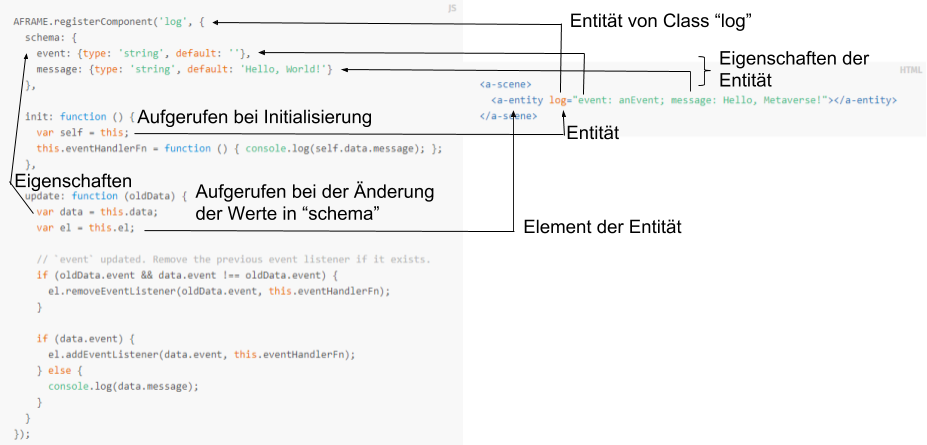
\includegraphics[width=\textwidth]{images/aframeClass.png}
\caption[typisches A-Frame Class]{typisches A-Frame Class}
\label{fig:aframeClass} 
\end{figure}
 
 Der Vorteil solcher Struktur ist, dass jede Entität eigne Kopie der Funktionen und Attribute von Component hat. Das bedeutet, dass ein Component(Class) viele Entitäten haben kann. Die Entitäten haben keine Beeinflussung mit einander.
 
 Allerdings muss die Struktur von Component wegen der Nutzung von Observer Pattern neu gestaltet werden.
 
 Wie der Code von Class \glqq Observable\grqq\ gezeigt, dass der Parameter der Funktion \glqq subscribe\grqq\ eine Funktion sein soll. Aber die Funktionen, die in Class definiert werden, gelten nicht als eine bestimmte Funktion bei JavaScript. Deshalb müssen die Funktionen, die als \glqq oberser\grqq benutzt werden, außer dem Class definiert werden, sodass die Entitäten von dem Class die Nachrichten von observable empfangen können. Das führt zu einer suboptimale Situation, dass alle Entität, die durch dem gleichen Class erstellt werden, dieselbe Funktionen und Eigenschaften benutzen.
 
 Obwohl die Struktur von Class passt sich die Philosophie von A-Frame nicht an, ist es praktisch und geeignet für diesem Projekt, weil fast alle Classes nur eine einzige Entiätit in der Szene haben.
 
 Um die Attribute und Funktionen von Component von die Funktion in \glqq observer\grqq\ zu erreichen, werden die Attribute und Funktionen beispielsweise schema auch außer dem Class als globale Variablen geschrieben.
 
\begin{figure}[ht]
\vspace*{0.3cm}
\centering
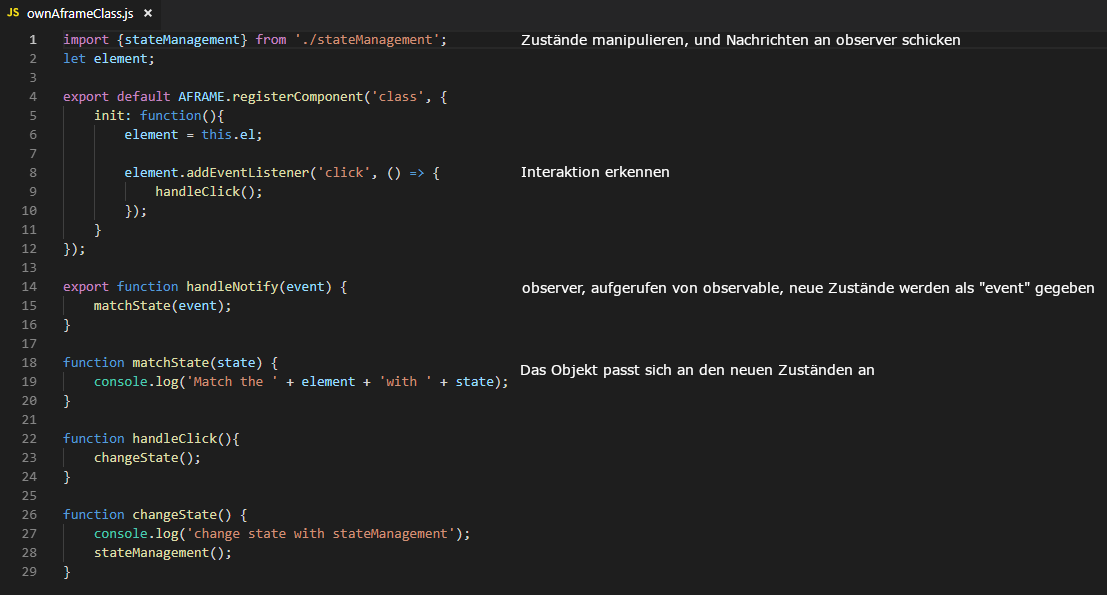
\includegraphics[width=\textwidth]{images/eigenesClass.png}
\caption[Eigene Class Struktur]{Eigene Class Struktur}
\label{fig:eigenesClass} 
\end{figure}
 
 \subsubsection{Möglichkeit der Verbesserung}
 Es ist auch möglich, nach der Philosophie von A-Frame die Class Struktur zu gestalten.
 
 Durch anpassend \glqq eventlistener\grqq\ (\glqq on\grqq\ in Jquery), die während der Initialisierung eingefügt wird, kann die Nachricht von \glqq observable\grqq\ in dem Class transportiert wird. (Abbildung ~\ref{fig:bestesClass})
 
\begin{figure}[ht]
\vspace*{0.3cm}
\centering
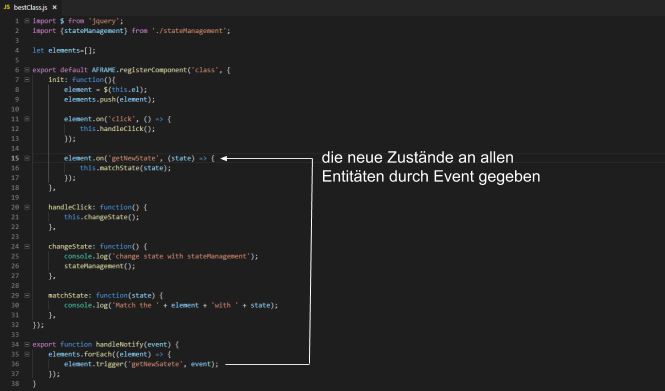
\includegraphics[width=\textwidth]{images/bestClass.png}
\caption[Bessere Class Struktur]{Bessere Class Struktur}
\label{fig:bestesClass} 
\end{figure}
 
 \subsection{Interaktion}
  Für unterschiedlichen Geräten werden entsprechend Interaktionen konzipiert. Die Implementierungen werden nach Geräten erzählt.
  
  \subsubsection{PC und Smartphone}
  Viele Interaktionen von PC und Smartphone werden durch selben Component umgesetzt, deswegen werden die Implementierung von PC und Smartphone zusammen erklärt.
  
  \textbf{Exploration}
  
  Mit einer Entität von built-in Component \glqq a-camera\grqq in A-Frame wird ein Kamera in der Szene eingesetzt. Dadurch wird die Sicht von Benutzer in der VR Umgebung erstellt. Die Interaktionen, die die Kamera betreffen, nämlich Exploration und Navigation werden in dieser Entität realisiert.
  
  Mit dem Component \glqq look-controls\grqq kann die Rotation einer Entität manipuliert werden. Wenn \grqq look-controls\grqq als Attribut von \glqq a-camera\grqq eingesetzt wird, wird es realisiert, die Drehung der Kamera zu manipulieren.
  
  Wenn die Eigenschaft \glqq pointerLockEnabled\grqq von \glqq look-controls\grqq  als \glqq true\grqq\ eingerichtet wird, wird der Zeiger auf PC durch ein Click auf Maus versteckt, und wird Kamera durch der Bewegung von Maus gedreht. Wenn ESC Taste auf Tastatur gedrückt wird, wird der Zeiger wieder gezeigt, und verliert der Maus die Kontrolle der Rotation der Kamera.
  
  Außerdem ist es möglich, durch das Ziehen auf dem Smartphone die Kamera zu drehen, wenn die Eigenschaft \glqq touchEnabled\grqq als \glqq true\grqq\ konfiguriert. \glqq true\grqq\ ist die Standardeinstellung für \glqq touchEnabled\grqq, deswegen muss das Attribut nicht extra eingerichtet werden.
  
  \textbf{Navigation}
  
  Mit dem Component \glqq wasd-controls\grqq kann die Position einer Entität manipuliert werden. Die Nutzung ist ähnlich wie das Component \glqq look-controls\grqq. Wenn \grqq wasd-controls\grqq als Attribut von \glqq a-camera\grqq eingesetzt wird, wird die Position der Kamera mit den Tasten W, A, S und D auf der Tastatur zu manipulieret.
  
  Die Eigenschaft \glqq acceleration\grqq beschreibt die Geschwindigkeit der Bewegung, wenn die Teste gedrückt. Um der Schwindel zu vermeiden, wird der Wert ziemlich klein eingerichtet.
  
  Es gibt noch Bug bei dem Component \glqq wasd-controls\grqq. Die manuelle Navigation kann mit Firefox richtig durchgeführt werden. Aber mit Chrome kann die Bewegung nicht beendet werden.
  
\begin{figure}[ht]
\vspace*{0.3cm}
\centering
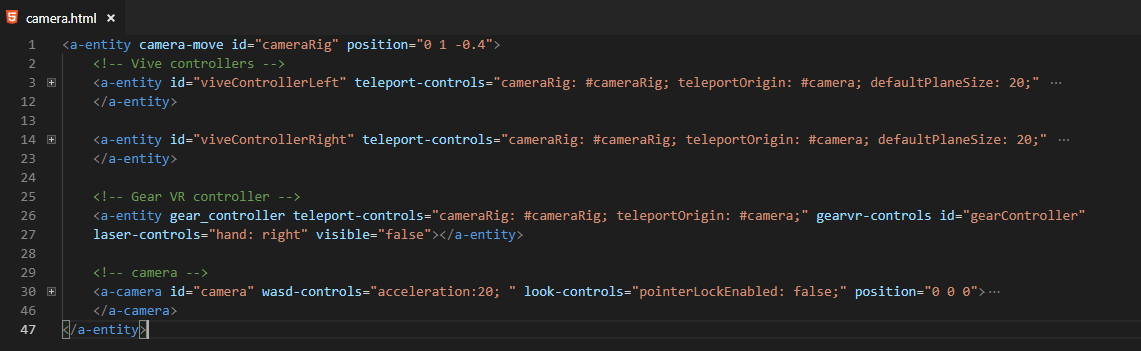
\includegraphics[width=\textwidth]{images/cameraHtml.png}
\caption[Kamera Element]{Kamera Element}
\label{fig:cameraHtml} 
\end{figure}
  
  Außer der manuellen Navigation wird auch die automatische Navigation implementiert. Das Event \glqq raycaster-intersected\grqq wird auf dasselbe Objekt emittiert, wenn das Objekt mit Zeiger überlappt. Dann bewegt sich die Kamera zu dem Objekt. Nach sechs Sekunden geht die Kamera wieder zurück. Wenn die Aktivitäten auf einem Objekt fertig sind, empfängt das Objekt keinem Event mehr. (Abbildung ~\ref{fig:cameraMove})
  
\begin{figure}[ht]
\vspace*{0.3cm}
\centering
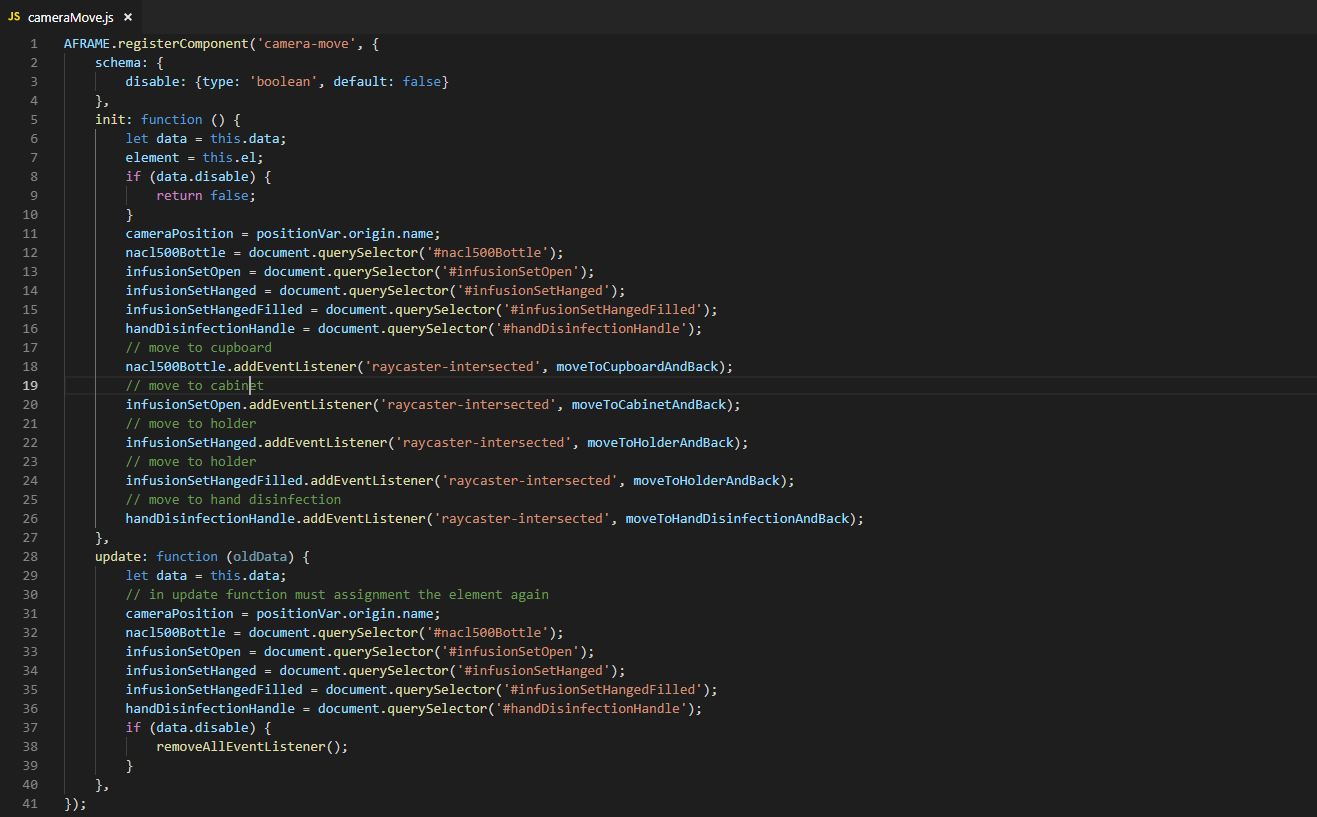
\includegraphics[width=\textwidth]{images/cameraMove.png}
\caption[Automatische Navigation]{Automatische Navigation}
\label{fig:cameraMove} 
\end{figure}
  
  \textbf{Manipulation}
  
  Die Manipulation auf PC und Smartphone wird mit dem built-in Component \glqq a-cursor\grqq implementiert. (Abbildung ~\ref{fig:aCursorElement}) Um der Zeiger in der Mitte der Sicht darzustellen, wird \glqq a-cursor\grqq als ein Child-Component von \glqq a-camera\grqq eingesetzt.
  
 \begin{figure}[ht]
\vspace*{0.3cm}
\centering
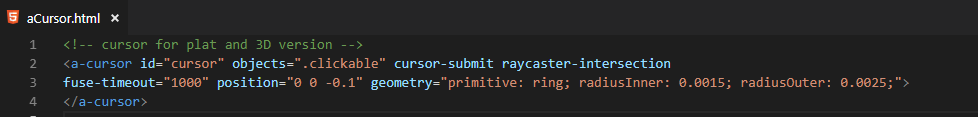
\includegraphics[width=\textwidth]{images/aCursorElement.png}
\caption[a-cursor Element]{a-cursor Element}
\label{fig:aCursorElement} 
\end{figure}
  
  Das Attribut \glqq objects\grqq beschreibt, mit welchen Objekten kann man interagieren. Alle solche Objekte werden mit Class \glqq clickable\grqq bezeichnet. Mit dem Attribut \glqq geometry\grqq wird der Zeiger als ein Ring definiert.
  
  Als Standardeinstellung wird der Zeiger auf PC aktiviert, wenn die linke Taste von der Maus gedruckt. Mit dem Attribut \glqq fuse-timeout\grqq wird der Zeiger auf Smartphone konfiguriert. Die Wert 1000 bedeutet, dass der Zeiger aktiviert wird, wenn der Zeiger auf einem Objekt 1 Sekunde fokussiert.
  
  Das Attribut \glqq raycaster-intersection\grqq ist eine Entität von Class \glqq raycaster-intersection\grqq, das die Funktion zu realisieren, dass der Zeiger zu grün wechselt, wenn der Zeiger die Objekte trifft, mit den interagieren kann.
  
  Das Event \glqq raycaster-intersected\grqq wird auf den Objekten selbe emittiert, wenn das raycaster sich mit den Objekten überlappt. Im Gegenteil wird \glqq raycaster-intersected-cleard\grqq emittiert, wenn nichts mit das Raycaster überlappt.
  
  Da \glqq a-cursor\grqq hat die Eigenschaften von Raycaster integriert, sind \glqq raycaster-intersection\grqq und \glqq raycaster-intersection-cleard\grqq für \glqq a-cursor\grqq zu Verfügung. (Abbildung ~\ref{fig:raycasterIntersection})
  
\begin{figure}[ht]
\vspace*{0.3cm}
\centering
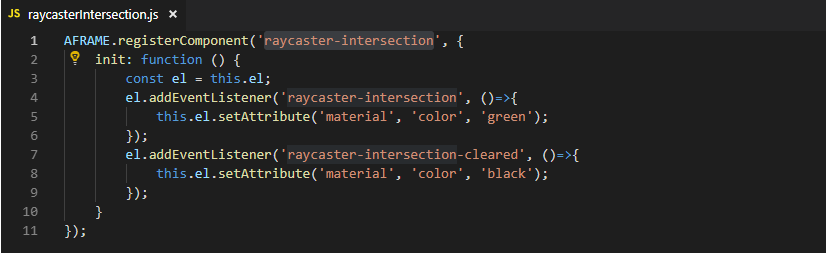
\includegraphics[width=\textwidth]{images/raycasterIntersection.png}
\caption[Automatische Navigation]{Automatische Navigation}
\label{fig:raycasterIntersection} 
\end{figure}
  
  Das Attribut \glqq cursor-submit\grqq ist zuständig für die Funktion, der Zeiger in Rot darzustellen und ein entsprechendes Geräusch zu klingen, wenn der Zeiger aktiviert wird. (Abbildung ~\ref{fig:cursorSubmit})
  
\begin{figure}[ht]
\vspace*{0.3cm}
\centering
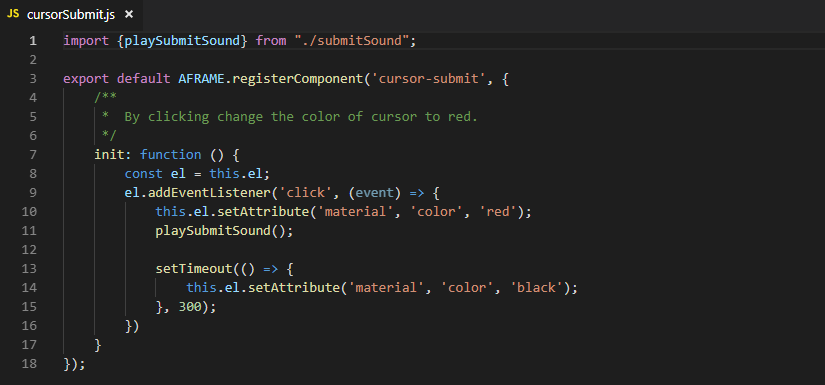
\includegraphics[width=\textwidth]{images/cursorSubmit.png}
\caption[Zeiger bestimmen]{Zeiger bestimmen}
\label{fig:cursorSubmit} 
\end{figure}
  
  \subsubsection{Samsung Gear VR}
  Die Interaktionen für Samsung Gear VR sind abhängig von der Verfügbarkeit des Controllers.
  
  \textbf{Ohne Controller}
  
  Die Interaktionen von Samsung Gear VR ohne Controller sollen von die Funktionen für PC und Smartphone durch A-Frame automatisch angepasst. Allerdings taucht ein Problem bei der Anpassung an Gear VR auf: die Zeiger für jede Auge überlappen sich nicht zusammen. Das heißt, dass zwei Zeiger in der Sicht erscheinen.
  
  Der Grund dafür ist, dass der Zeiger zu nahe zu der Augen. Wenn der Zeiger weiter zu der Augen gelegt wird, ist der Zeiger eindeutig. Jedoch das führt zu der Situation, dass der Zeiger hinter dem Objekt wie Krankenakte ist. Wenn die Krankenakte auch weiter eingesetzt wird, können die Informationen auf der Krankenakte nicht deutlich gesehen werden.
  
  Zwei mögliche Lösungen werden versucht, Raycaster und große Skalierung.
  \begin{itemize}
      \item \textbf{Raycaster}: Die Idee Raycaster ist, das Raycaster von Controller zu den Augen zu bringen. Der Zeiger ist nicht mehr ein Ring, sondern eine aus Augen ausstrahlende Linie, sodass der Abstand zwischen Augen und Objekte keine Rolle spielt. Allerdings wird das Raycaster in Gear VR nicht richtig dargestellt. Die Linie wird als viele kurze Stückchen geschnitten. Und die Stückchen zeigen nicht nach einer bestimmen Richtung. (Abbildung ~\ref{fig:GearVRRaycaster})
      
\begin{figure}[ht]
\vspace*{0.3cm}
\centering
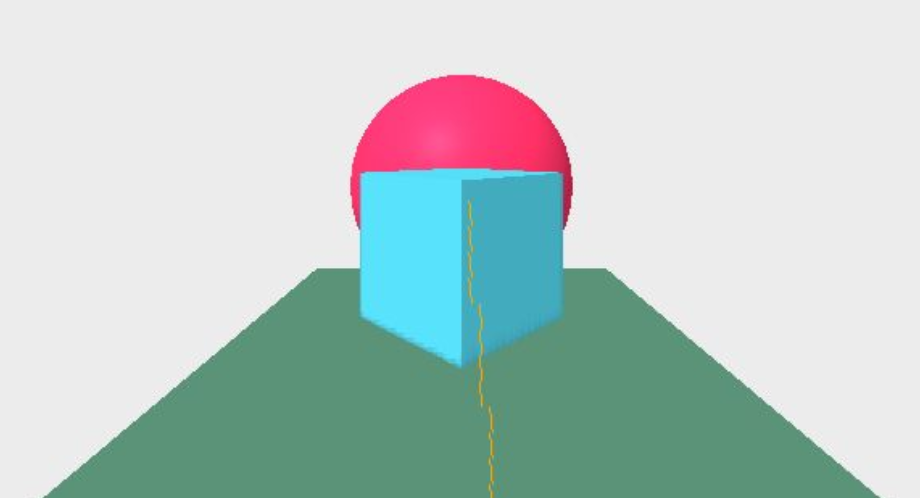
\includegraphics[width=\textwidth]{images/gearVRRaycaster.png}
\caption[Raycaster in Gear VR]{Raycaster aus Kamera in Gear VR in A-Frame basic Scene}
\label{fig:GearVRRaycaster} 
\end{figure}
      
      \item \textbf{große Skalierung}: Der Zeiger und die andere Objekte werden weit gelegt. Um die Objekten deutlicher zu schauen, werden alle Objekten vergrößern, sodass die relative Große sich nicht verändert. Die Position der Kamera wird dafür angepasst.
      (Abbildung ~\ref{fig:GearVRCursor})
      
\begin{figure}[t]
\vspace*{0.3cm}
\centering
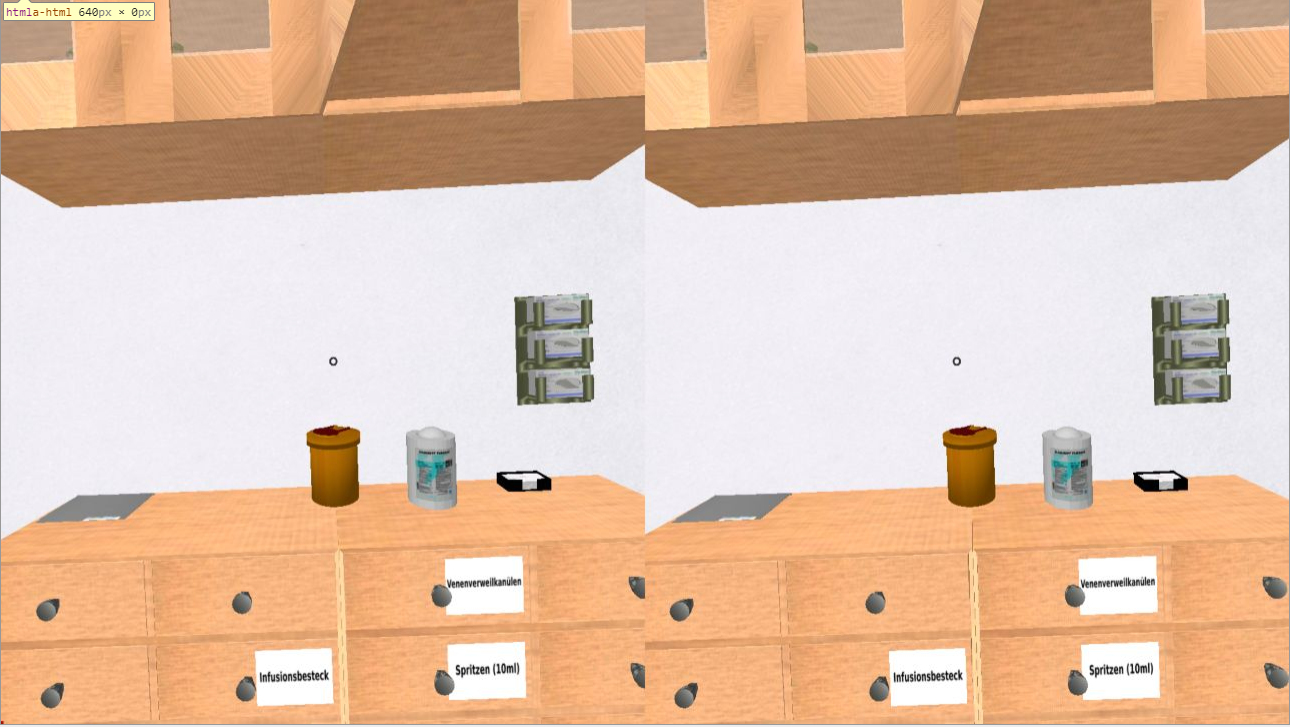
\includegraphics[width=\textwidth]{images/gearVRCursor.png}
\caption[vergrößerte Szene in Gear VR]{vergrößerte Szene in Gear VR}
\label{fig:GearVRCursor} 
\end{figure}
      
  \end{itemize}
  
  Obwohl die zweite Möglichkeit keine optimale Lösung ist, weil der Benutzer sich fühlt, dass selbe ein Gigant ist, ist es besser als Raycaster, deswegen wird diese Lösung eingesetzt. 
  
  \textbf{Mit Controller}
  
  Die Navigation und Manipulation werden durch den Controller aktiviert.
  
  Das Element von Gear VR Controller wird mit dem Element von Kamera zusammen in dem Element mit ID \glqq cameraRig\grqq\ eingepackt. Die Bewegung der Kamera wird durch die Translation von \glqq cameraRig\grqq\ geschafft, sodass wird die relative Position zwischen der Kamera und dem Controller während der Bewegung behaltet.
  
  Mit dem built-in Component \glqq teleport-controls\grqq\ werden die Navigation implementiert. Das Attribut \glqq cameraRig\grqq\ beschreibt das Element, das sich zu der bezeichneten Position bewegt. Das Attribut \glqq teleportOrigin\grqq\ beschreibt das Element, das als die Ursprung von dem Element \glqq cameraRig\grqq\ gilt.
  
  Wenn der Trackpad auf Gear VR Controller gedrückt wird, wird die Position bezeichnet. Solange der Trackpad losgelöst wird, bewegt sich das Element \glqq cameraRig\grqq\ zu der bezeichneten Position. Die Position der Kamera auf den X und Z Achsen sind gleich wie die bezeichnete Position.
  
  Die Manipulation wird durch dem Component \glqq laser-controls\grqq\ realisiert. Mit dem Component wird nicht nur der Gear VR Controller, sondern auch Daydrame Controller usw. (Abbildung ~\ref{fig:GearVRControllerElement} \& Abbildung ~\ref{fig:GearVRWithController})
  
\begin{figure}[ht]
\vspace*{0.3cm}
\centering
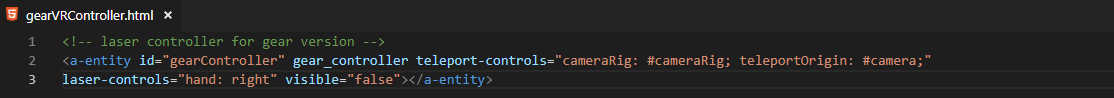
\includegraphics[width=\textwidth]{images/gearVRControllerElement.png}
\caption[Gear VR Controller Element]{Gear VR Controller Element}
\label{fig:GearVRControllerElement} 
\end{figure}
  
\begin{figure}[ht]
\vspace*{0.3cm}
\centering
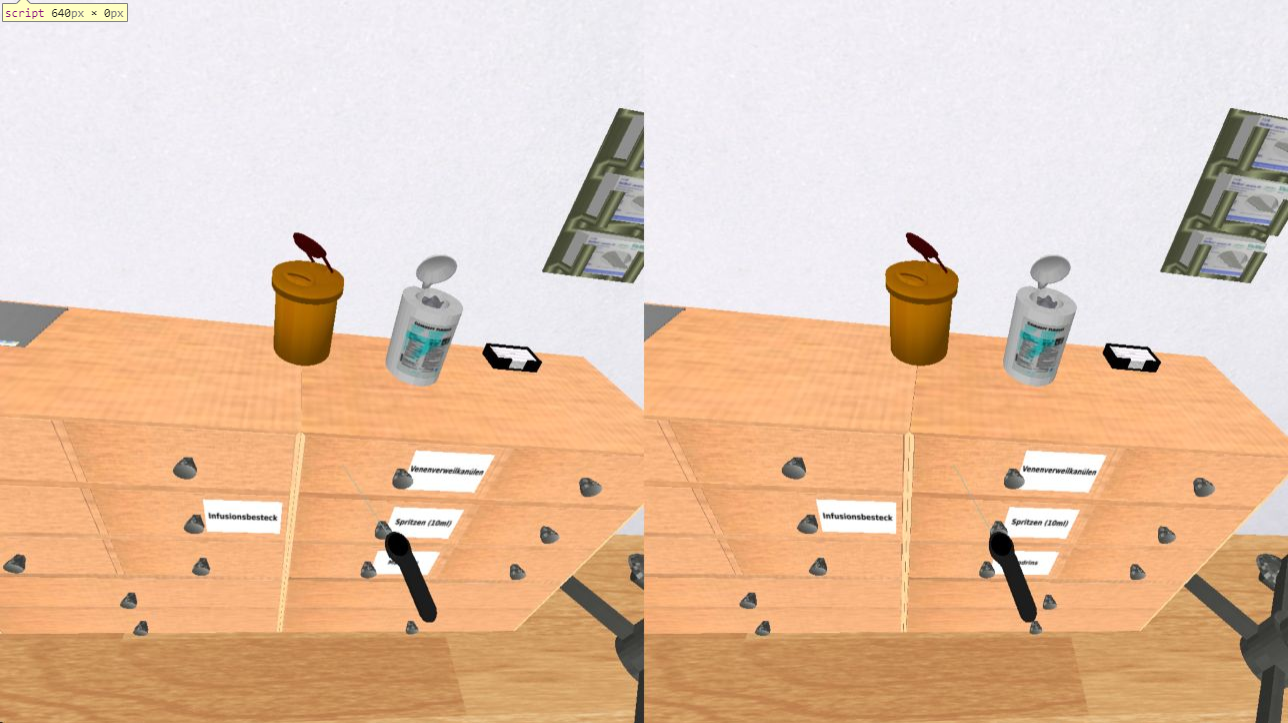
\includegraphics[width=\textwidth]{images/gearVRWithController.png}
\caption[Gear VR mit Controller]{Gear VR mit Controller}
\label{fig:GearVRWithController} 
\end{figure}
  
  \subsubsection{HTC Vive}
  
  Die Navigation von HTC Vive wird durch dem Component \glqq teleport-controls\grqq\ gleich wie Gear VR implementiert.
  
  \textbf{Component vive-controls}
  
  Durch dem built-in Component \glqq vive-controls\grqq\ werden die Vive Controllers anerkannt. Mit dem Attribut \glqq model\grqq\ wird die Darstellung des Modells von Controller konfiguriert. Da der Controllers als Hände gezeigt, wird das Attribut als \glqq false\grqq\ eingerichtet. (Abbildung ~\ref{fig:viveControllerElement})
  
\begin{figure}[ht]
\vspace*{0.3cm}
\centering
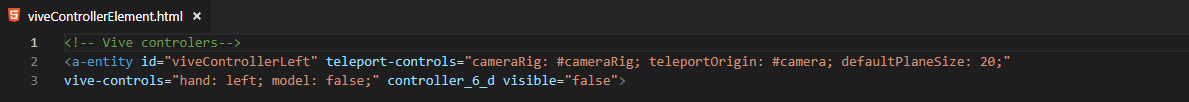
\includegraphics[width=\textwidth]{images/viveControllerElement.png}
\caption[Vive Controller Element]{Vive Controller Element}
\label{fig:viveControllerElement} 
\end{figure}
  
  Nach der Erkennung der Controllers werden Events \glqq triggerdown\grqq\ und \glqq triggerup\grqq\ ausgelöst, wenn der Auslöser gedrückt und losgelöst. Um die Nachrichten über die Aktivität der Controllers auszubreiten, wird Observer Pattern verwendet.
  
  Die Controller relevante Funktionen bei unterschiedlichen Objekten melden sich bei den Observerables für \glqq triggerdown\grqq\ und \glqq triggerup\grqq\ an. Wenn der Auslöser gedrückt oder losgelöst, wird die Informationen(Name von Event, ID von Controller, globale Position von Controller) an alle Observers geschickt.(Abbildung ~\ref{fig:controller6D})
  
\begin{figure}[ht]
\vspace*{0.3cm}
\centering
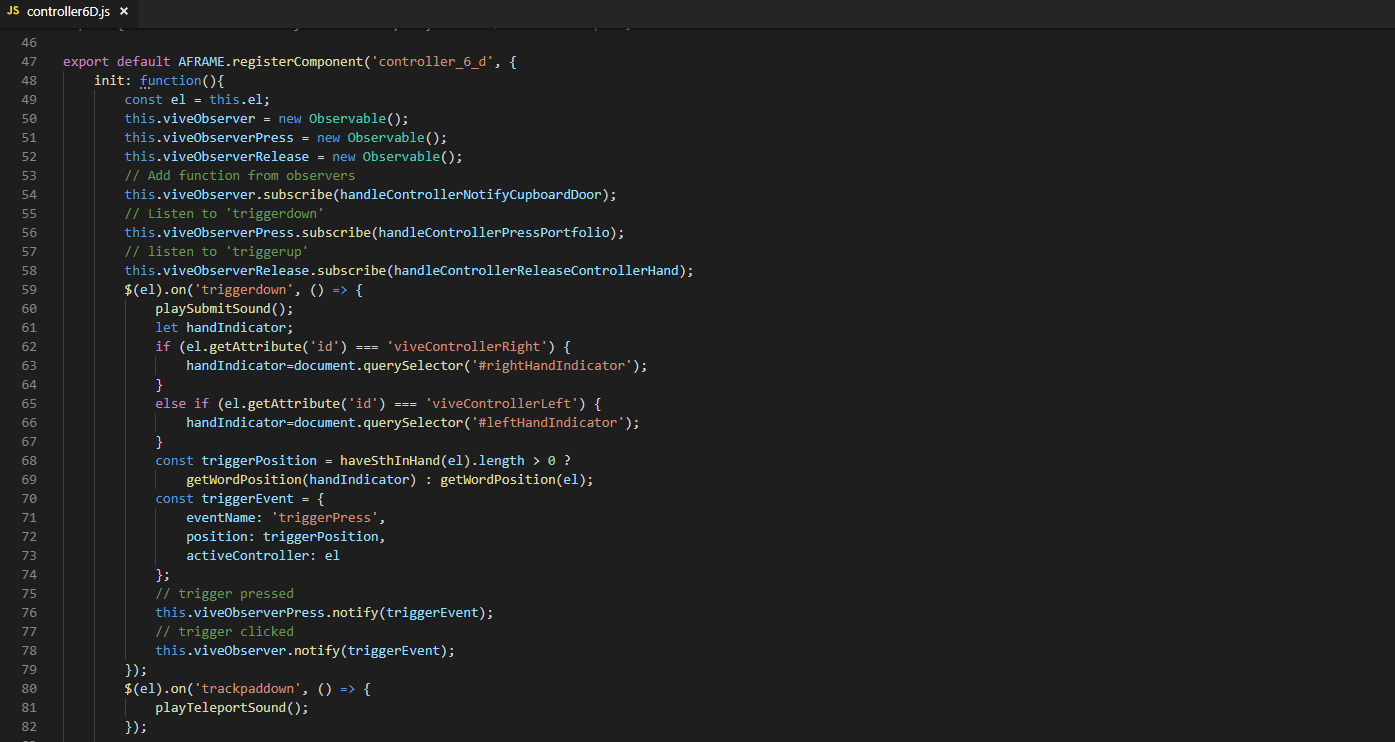
\includegraphics[width=\textwidth]{images/controller6D.png}
\caption[6 DoF Controller]{6 DoF Controller}
\label{fig:controller6D} 
\end{figure}
  
  Um die globale Position zu rechnen, wird die Funktion von three.js verwendet. Die A-Frame Objekte sind eigentliche verpackte three.js Objekte, deswegen ist die Verwendung von three.js in A-Frame barrierefrei. Das gilt als ein Vorteil von A-Frame. (Abbildung ~\ref{fig:getWorldPosition})
  
\begin{figure}[ht]
\vspace*{0.3cm}
\centering
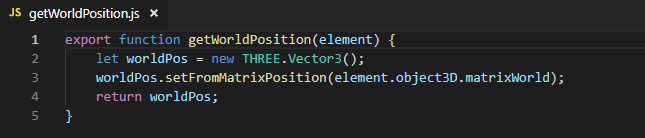
\includegraphics[width=\textwidth]{images/getWorldPosition.png}
\caption[get global position]{get global position}
\label{fig:getWorldPosition} 
\end{figure}
  
  \textbf{Prüfung mit Raycaster}
  
  Ein aus Augen ausstrahlendes verstecktes Raycaster in dem Element \glqq a-camera\grqq\ eingesetzt. Wenn die Krankenakte, Infusionsflasche und Infusionsbesteck überprüft werden sollen, wird das Raycaster gezeigt, um die Überprüfung durchzuführen. Wenn das Raycaster die richtige Position trifft, Event \glqq raycaster-intersection\grqq\ ausgelöst wird, wird das Raycaster in grün dargestellt, sonst in orange. Wenn die Überprüfung fertig ist, die relevante Zustände für die Prüfungen als \glqq true\grqq\ gesetzt, wird das Raycaster wieder versteckt.
  
  \textbf{Zustände für Vive Controller}
  
  Weil die Manipulation mit Vive Controller große Freiheit hat, und nicht jede Ausführung einer Aktivität den Fortschritt fördert, werden eine neue Liste für die Zustände der Vive Controllers und die entsprechenden Funktionen erstellt.
  
  Zum Beispiel wird der Wert des Zustands für Vive Controller \glqq portfolioInHand\grqq\ als die ID des Controllers, der mit der Krankenakte interagiert, gespeichert, und die Zustände an die Observers(Krankenakte usw.) geschickt. Solange die Änderung des Zustands im Component Krankenakte informiert wird, wird das Element der Krankenakte in dem Element des entsprechenden Controllers eingezogen. (Abbildung ~\ref{fig:controller6D} \& Abbildung ~\ref{fig:portfolioPress})
  
\begin{figure}[ht]
\vspace*{0.3cm}
\centering
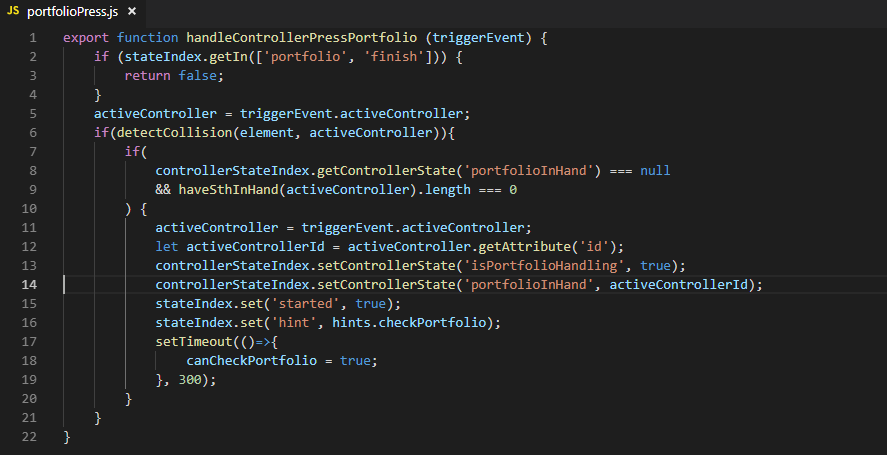
\includegraphics[width=\textwidth]{images/portfolioPress.png}
\caption[Bearbeitung der Krankenakte]{Bearbeitung der Krankenakte}
\label{fig:portfolioPress} 
\end{figure}
  
  \textbf{Attribute Veränderung}
  
  Wenn ein Element in dem Controller Element eingezogen oder aus dem Controller ausgezogen wird, wird die Dimension der Koordination geändert. Deshalb muss das Attribut Position neu gerechnet und umgesetzt.
  
  Normalerweise kann das Attribut direkt mit dem Befehl \glqq setAttribute\grqq konfiguriert werden. Allerdings sind die 3D A-Frame Objekte viel größer als 2D Objekte, sodass die DOM Manipulation länger dauert. Deshalb passiert es, dass die Änderung des Attributs vor dem Umzug des DOM Elements geschafft wird. Und nach dem Umzug wird das Attribut wieder zurückgesetzt.
  
  Um das Problem zu lösen, muss die DOM Funktion \glqq MutationObserver\grqq\ verwendet. Die Funktion \glqq MutationObserver\grqq\ ist zuständig dafür, die Änderung der gegebenen Attribute eines Elements zu beobachten. Wenn die Änderung fertig ist, wird eine Nachricht an den allen Observers geschickt.
  
  Weil die DOM Manipulation sehr häufig ist und fast alle aufwendige Änderungen mit den Controllers zu tun haben, wird die Funktion \glqq MutationObserver\grqq\ in einem Class \glqq controllerActions\grqq\ verpackt, um die Verwendung zu vereinfachen.
  
  Die \glqq MutationObserver\grqq\ beachtet die \glqq childList\grqq\ des eingegebenen Controllers. Wenn die Einfügung und Entfernung der Child Elements des Controllers fertig ist, werden die eingegebenen Attribute eingesetzt. 
  
  image: controllerAction .........
  
  \textbf{Hinweis-Box}
  
  Die Hinweis-Box wird durch das built-in Element \glqq a-box\grqq\ implementiert. Durch die Konfiguration des Attributs \glqq material\grqq\ wird die Hinweis-Box in halb transparentem Rot dargestellt, wenn ein Objekt beispielsweise Krankenakte in Hand ist. Die Hinweis-Box hört zu den Zuständen aller Objekte. Wenn alle nötige Aktivitäten für das Objekt fertig gemacht, z.B. Überprüfung der Krankenakte, werden die Änderungen der entsprechenden Zuständen von der Hinweis-Box erkannt. Nach der Erkennung wird das Attributs \glqq material\grqq\ zum Grün umgeschrieben.
  
  Wenn die Kollision zwischen der grüne Hinweis-Box und dem Objekt in Hand während des Loslösens auf den Auslöser des Controllers detektiert wird, wird der entsprechende Zustand geändert und das Objekt auf den entsprechend Platz gelegt.
  
  image: code HTML toggleBoxPortfolio .........
  image: code class toggleBoxPortfolio .........
  
  \textbf{Kollisionserkennung}
  
  Die Funktion Kollisionserkennung wird durch die Funktionen von three.js implementiert. Die zwei Objekte werden erst durch die Funktion \glqq setFromObject\grqq\ als Kuben umgerechnet. Durch die Funktion \glqq intersectsBox\grqq\ wird es überprüft, ob zwei Kuben überlappt sind, damit die Kollision zu erkennen.
  
  Allerdings ist die Methode keine optimale Lösung. Wenn der Rahmen des Objektes kein Kubus ist, ist die Kollisionserkennung ungenau.
  
  image: code collision detection.
  
  \textbf{Freier Fall}
  
  Die Objekte können aus den Händen fallen, wenn der Auslöser losgelöst wird.
  
  Das Fallen wird so simuliert, dass in jedem bestimmten Zeitraum (z.B. 0.01 Millisekunde) die Position auf Y Achse des Objektes eine Geschwindigkeit reduziert wird. Laut der Formel der Geschwindigkeit des freien Falls 
  
  image: Formel Geschwindigkeit V(t) = gt, g = 9.8 .........
  
  kann die Geschwindigkeit so gerechnet \textit{speed = speed + accelerate} werden. 
  
  Da das reale Schwerefeld ist 9.8 m/s, soll die konstante Wert \textit{accelerate} 0.098 sein. Aber in der simulierten VR Umgebung fällt das Objekt zu schnell, sodass das Fallen nicht deutlich gemerkt werden kann. Um bessere Benutzererfahrung zu implementieren, wird die Wert \textit{accelerate} als 0.049 befestigt.
  
  Um der passende Zeitpunkt zu finden, das Fallen zu beenden, wird jede 0.01 Millisekunde die Kollision auf Y Achse detektiert. Allerdings könnte es passieren, dass vor der Detektion das Objekt in der letzten 0.01 Millisekunde schon in anderem Objekt beispielsweise Boden gefallen. Wenn das Objekt sehr dünn ist, z.B. Namenetikett, wird es nicht mehr gesehen.
  
  Um das Problem zu vermeiden, wird eine Variable \textit{lowestY} benutzt. Damit kann eine neue Ebenen erstellte werden, die als eine Kollision Ebene auf Y Achse gilt. Mit der Hilfe der neuen Ebenen, kann das Fallen des Objektes früher beendet werden. Allerdings kann es passieren, dass das Objekt über dem Boden liegt.
  
  Außer Boden (Y = 0) können andere Objekte wichtige Rolle bei dem Fallen spielen, z.B die Arbeisoberfläche auf den Schubladentisch. Um der Bereich der Arbeitsoberfläche zu finden, muss die Koordination des Rahmen des Schubladentisches in der Szene gefunden werden. Das A-Frame Objekt wird erst zum three.js Box3 Objekt umgesetzt. Der Wert der Position des Rahmens des Objektes kann aus der Eigenschaft \glqq boundingBox\grqq gefunden werden. Die höchste Fläche gilt als die Kollision Bereich.
  
  image: code getWordBound, handleSpecialCondition .........
  
  \subsubsection{Möglichkeit der Verbesserung}
  Die kürzere Ladezeit der Applikation führt zur besseren Benutzererfahrung. Die Größe der Dateien spielt wichtige Rolle bei der Ladung.
  
  Nicht alle Geräten mit HTC Vive verbinden, deswegen es wäre besser, dass die Codes, die mit HTC Vive zu tun haben, in eigne Datei geschrieben und in einem Verzeichnis gespeichert werden sollen. Dieses Verzeichnis wird geladen, nur wenn die HTC Vive Controllers erkannt werden.
  
  Sodass wird die Ladezeit für die Geräten außer HTC Vive verringert.
  
 \subsection{Geräte anpassen}
 Anpassende Interaktionen werden für unterschiedlichen Geräte gestaltet und implementiert. Um die Szene lebendig darzustellen, die Interaktion barrierefrei durchzuführen und die falsche Initialisierung der Position der Kamera(Bug von A-Frame) zu beheben muss die Applikation für unterschiedlichen Geräten während des Ladens konfiguriert wird.
 
 Durch die Funktion \glqq navigator.userAgent\grqq wird die Informationen über dem Browser ausgelesen. Dadurch wird die Typen der Geräten(PC, Smartphone, GearVR) unterschieden. Durch das Event \glqq gamepadconnected\grqq wird der verbundene Controller(GearVR Controller, Vive Controller) erkannt. Damit wird die Mode auf PC(flach, VR) und Gear VR(ohne Controller, mit Controller) unterschieden. Durch das Event \glqq enter-vr\grqq\ wird die Mode auf Smartphone(flach, Cardboard) unterschieden.
 
 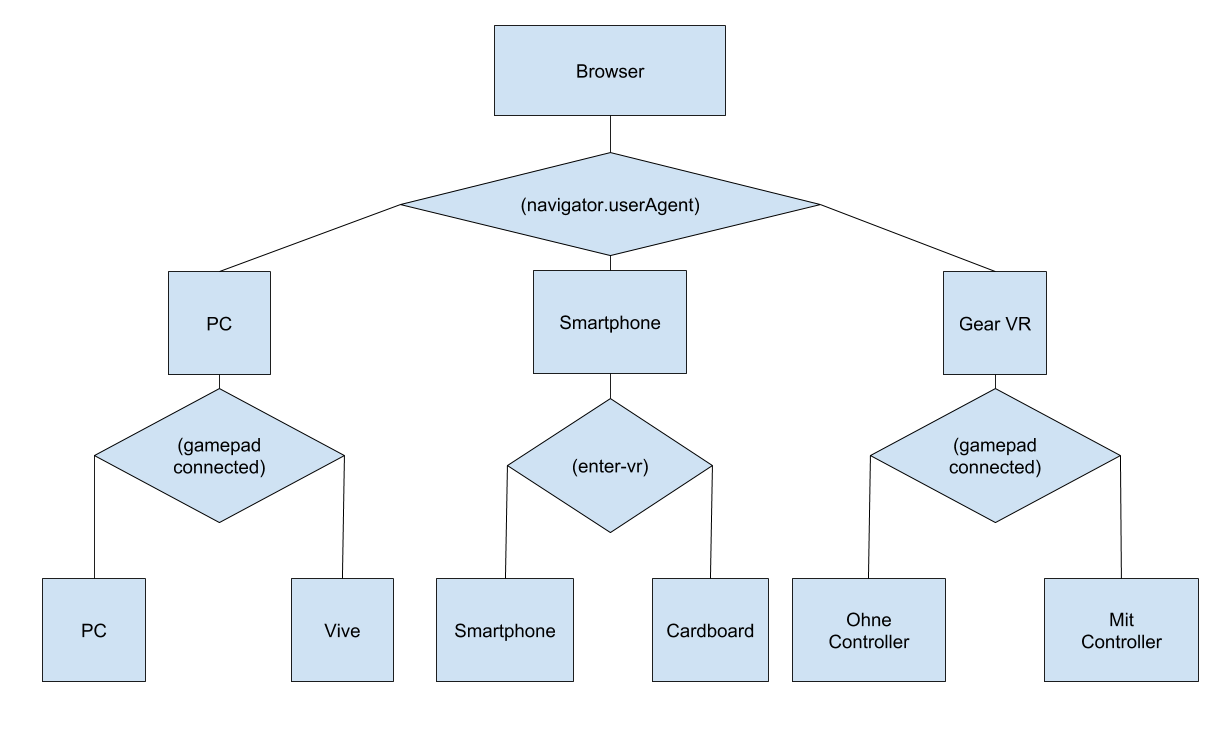
\includegraphics[width=\textwidth]{images/geraeteAnpassen.png}

\begin{table}
\centering
\begin{tabular}{|l|l|l|l|l|l|} 
\toprule
PC & Vive                                                                         & \begin{tabular}[c]{@{}l@{}}Smart-\\phone\end{tabular} & Cardboard                                                           & \begin{tabular}[c]{@{}l@{}}Ohne\\Controller\end{tabular}             & \begin{tabular}[c]{@{}l@{}}Mit\\Controller\end{tabular}                       \\ 
\hline
   & Ring Zeiger entfernen                                                        &                                                       & \begin{tabular}[c]{@{}l@{}}Kamera Position\\einstellen\end{tabular} & \begin{tabular}[c]{@{}l@{}}Objekte \\skarlieren\end{tabular}         & Ring Zeiger entfernen                                                         \\ 
\cline{2-2}\cline{4-6}
   & Objekte skalieren                                                            &                                                       &                                                                     & \begin{tabular}[c]{@{}l@{}}Kamera Position~\\einstellen\end{tabular} & \begin{tabular}[c]{@{}l@{}}Automatische Bewegung \\deaktivieren\end{tabular}  \\ 
\cline{2-2}\cline{5-6}
   & \begin{tabular}[c]{@{}l@{}}Kamera Position \\einstellen\end{tabular}         &                                                       &                                                                     &                                                                      & Objekte skalieren                                                             \\ 
\cline{2-2}\cline{6-6}
   & \begin{tabular}[c]{@{}l@{}}Automatische Bewegung \\deaktivieren\end{tabular} &                                                       &                                                                     &                                                                      & \begin{tabular}[c]{@{}l@{}}Gear VR Controller \\darstellen\end{tabular}       \\ 
\cline{2-2}\cline{6-6}
   & \begin{tabular}[c]{@{}l@{}}Vive Controller \\darstellen\end{tabular}         &                                                       &                                                                     &                                                                      &                                                                               \\
\bottomrule
\end{tabular}
\caption{Anpassung der Geräten}
\end{table}
 
 \subsection{Töne}
 Die Töne sind wichtig, eine lebendige Simulation aufzubauen. Alle realen Geräusche werden während der Übung in reale Skillslab in Fachhochschule Bielelfeld aufgenommen. Die Größe ist ca. 14 MB. Es ist zu groß in einer webbasierte Applikation einzufügen, weil es zu lange Zeit für das Laden führt. Deswegen werden nur die Geräusche für die Feedbacks von Controllers eingesetzt.
 
 Vier Geräusche werden bei der Kamera eingesetzt, und für den Druck und die Loslösung auf dem Auslöser und dem Trackpad angepasst. Die built-in Funktion \glqq playSound\grqq\ wird in dem Objekt \glqq sound\grqq\ von \glqq componets\grqq\ eingepackt. Wenn ein Event von Controllers emittiert wird, wird die Funktion \glqq playSound\grqq\ des entsprechenden Sound Objekt aufgerufen.
 
 image: code submitSound .........
 
 \subsection{Arbeitsoberfläche Desinfektion in Vive}
 Das Feedback der Desinfektion der Arbeitsoberfläche wird durch eine Hinweis-Box über dem Mülleimer und zwei versteckte Umschalter auf der Arbeitsoberfläche implementiert.
 
 Solange ein Desinfektionstuch in Hand genommen wird, wird eine rote Hinweis-Box über dem Mülleimer dargestellt, um die Botschaft zu vermitteln, dass das Tuch und Handschuhe in dem Mülleimer eingeworfen werden sollen, aber zur Zeit die Voraussetzung(Desinfektion der Arbeitsoberfläche) noch nicht erfüllt wird.
 
 Gleichzeitig überprüfen die zwei Umschalter jede 0.5 Sekunde, ob die Kollision zwischen dem Tuch und den Umschalter erkannt wird. Wenn ein Schalter mit dem Tuch getroffen hat, wird der entsprechende Zustand für Vive Controller als \glqq true\grqq\ umgesetzt.
 
 Solange die beiden Zustände der Umschalter \glqq true\grqq\ sind, wechselt die Farbe der Hinweis-Box über dem Mülleimer zum Grün, um die Information zu teilen, dass das Tuch und die Handschuhe in dem Mülleimer einwerfen dürfen.
 
 image: code tuch, szene .........
 
 \subsection{Animation}
 Die Animation in A-Frame wird auch durch ein HTML Element \glqq a-animation\grqq bezeichnet. Das übergeordnete Element ist das Objekt zu animiert. Die genaue Manipulation wird durch die Attribute des \glqq a-animation\grqq Elements konfiguriert. Hier werden die wichtige Attribute aufgellist:
 
 image: beispiel html animation element .........
 
\begin{table}
\centering
\begin{tabular}{lll} 
\toprule
Name      & Beschreibung                                                                                                          & Standardeinstellung  \\
attribute & Das Attribut des übergeordneten Elements zu animieren                                                                 & rotation             \\
begin     & Name des Events, die Animation aufzurufen                                                                             & ''                   \\
from      & Die Wert am Anfang                                                                                                    &                      \\
to        & Die Wert am Ende                                                                                                      &                      \\
dur       & Die Zeitdauer der Animation                                                                                           & 1000                 \\
direction & Die Richtung der Animation (zwischen Anfang und End)                                                                  & normal               \\
fill      & \begin{tabular}[c]{@{}l@{}}Der Effekt der Animation zu bestimmen, \\wenn die Animation deaktiviert wird.\end{tabular} & forwards             \\
repeat    & Die Zahl der Wiederholung der Animation                                                                               & 0                    \\
easing    & Die Erleichterung der Animation                                                                                       & ease                 \\
\bottomrule
\end{tabular}
\caption{Wichtige Attribute von a-animation Element}
\end{table}
 
 Um die Animation einfach zu benutzen, wird eine Funktion entwickelt. Das \glqq a-animation\grqq Element wird erstellt. Und nach dem Laufen der Animation wird das Element nach dem Bedarf, der als Parameter eingegeben, entworfen oder behaltet.
 
 image: code animation .........
 
 
 \subsection{Hand}
 
 Durch das \glqq a-animation\grqq Element kann ganzes Objekt animiert werden. Um komplizierte Animation zu realisieren, wird das Objekt während der Modellierung direkt animiert.
 
 Das Hand Modell wird in Blender animiert. Zuerst wird das Skelett für die Hand erstellt. Mit die Funktion \glqq Set Parent To \grqq\ können das Modell und die Skelett zusammen verbinden. Durch \glqq Key Frame\grqq\ kann die Hand animiert werden.
 
 image: bledner hand .........
 
 Das Modell wird als glTF 2.0 exportiert. Das glTF 2.0 ist ein Format für 3D Objeket, die für webbasierte Applikation entwickelt. Die Vorteile sind kleine Größe und die Unterstützung der Animation.
 
 Bei A-Frame kann die Animation durch das Attribut \glqq animation-mixer\grqq\ von dem Hand Modell aufgerufen werden. Allerdings kann der Zeitraum der Animation bei A-Frame nicht ausgewählt werden, was mit Unity oder Unreal Engine geschafft werden kann. Deshalb kann der Effekt, dass die Hand Faust während des Drucks auf dem Auslöser ein bisschen macht und die Hand Faust während der Auslösung auf den Auslöser lockert, nicht implementiert werden.
 
 image: code animation-mixer .........
 
 
 \subsection{Uhr}
 
 Die Uhr hat zwei Funktionen in der Szene, die Uhrzeit darzustellen und der 30 Sekunden Markierung während der Händedesinfektion zu zeigen.
 
 \subsubsection{Uhrzeit darstellen}
 Um die reale Uhrzeit darzustellen, wird ein Class \glqq clock\_hand\_roll\grqq\ entwickelt. Da der Zeiger bewegt sich jede Sekunde, wird die built-in Funktion \glqq tick\grqq\ benutzt. Die von \glqq tick\grqq\ aufgerufene Funktionen werden jede Sekunde ein Mal durchgeführt, wie \glqq setInterval\grqq\.
 
 Mit der Hilfe der Funktion \glqq tick\grqq\ wird jede Sekunde das Attribute \glqq Rotation\grqq\ der allen drei Zeiger aktualisiert. 
 
 Um der Winkel der Rotation zu rechnen wird zuerst die aktuelle Uhrzeit durch das Class \glqq Data\grqq\ bekommen. Und mit den Funktionen \glqq getSeconds\grqq\, \glqq getMinutes\grqq\, \glqq getHours\grqq\ werden die Ziffern für jeden Zeiger gerechnet.
 
 Danach wird der Winkel jedes Zeigers gerechnet, der bei jeder Bewegung dreht. Für Sekundenzeiger und Minutenzeiger ist der Winkel 360/60. Für Stundenzeiger ist der Winkel 360/12.
 
 Das Produkt von der Ziffer mal entsprechendem Winkel bei jeder Bewegung ist der Winkel der Rotation auf X Ebene in der Koordination.
 
 image: code Uhr....
 
 \subsubsection{30 Sekunden Markierung}
 Solange der Griff des Händedesinfektionsspenders gedrückt wird, wird ein Event \glqq handwashing\grqq\ emittiert. Danach wird ein A-Frame Element \glqq a-gltf-model\grqq\ für die 30 Sekunden Markierung mit entsprechenden Attributen  erstellt. Die Methode, die Rotation zu rechnen, ist gleich wie die Methode für den Sekundenzeiger. Nach 30 Sekunden wird das Markierung Element entworfen.
 
 image: 30 sekunden Markierung
 
 
 \subsection{Transparenz}
 

